\documentclass[../EngineeringJournal_CDavis.tex]{subfiles}

\begin{document}

%%%%%%%%%%%%%%%%%%%%%%%%%%%%%%%%%%%%%%%%%%%%%%%%%%%%%
%%%%%%%%%%%%%%%%%%%%%%%%%%%%%%%%%%%%%%%%%%%%%%%%%%%%%

\chapter[Configuring Vlans and Trunks]{Configuring Vlans\linebreak[1] and
Trunks \hspace*{\fill March 4, 2020}}
\noindent\textbf{{Packet Tracer Lab 13} \hspace*{\fill}{\textbf{CIT 167}}}\linebreak[1]
{{Spring 2020} \hspace*{\fill}{Chaz Davis}}                             
%===================================
%===================================


\hspace{0.2cm}
\begin{tcolorbox}[width=6.3in]
\scriptsize 
vlans and trunks
  \begin{outline}
    \1 configure terminal
    \1 interface interface-id
    \1 switchport mode {dynamic {auto | desirable} | trunk}
    \1 switchport access vlan vlan-id
    \1 switchport trunk native vlan vlan-id end
    \1 show interfaces interface-id switchport
    \1 show interfaces interface-id trunk
    \1 copy running-config startup-config
  \end{outline}
\end{tcolorbox}
\hspace{0.2cm}
\normalsize  
  
\clearpage

%===================================
\mysection{\textbf{Part 1: Configuration}}

I set up the configurations for each pc on the network. 


\begin{figure}[!hbt]\centering
\subfloat[PC3 Configuration]{\label{PCConfig13PC3}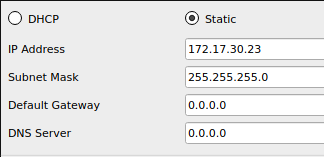
\includegraphics[width=.45\linewidth]{Figures/2020-03-19-172951_324x157_scrot.png}}\par
\subfloat[PC4 Configuration]{\label{PCConfig13PC4}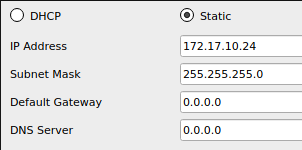
\includegraphics[width=.45\linewidth]{Figures/2020-03-19-173054_302x150_scrot.png}}\hfill
\subfloat[PC6 Configuration]{\label{PCConfig13PC6}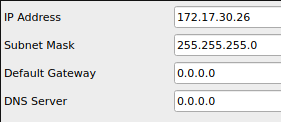
\includegraphics[width=.45\linewidth]{Figures/2020-03-19-173105_281x122_scrot.png}}\par
\caption{PC configurations}\label{PCConfig13}
\end{figure}


I then copied and pasted the commands from the handout for each of the
switches:


\begin{figure}[!hbt]\centering
\subfloat[show ip int brief on Switch 2]{\label{Show13Ip2}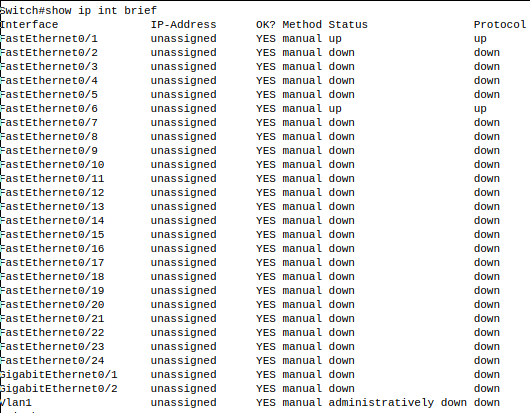
\includegraphics[width=.45\linewidth]{Figures/2020-03-19-180321_530x413_scrot.png}}\hfill
\subfloat[show vlan brief on Switch 2]{\label{Show13Vlan2}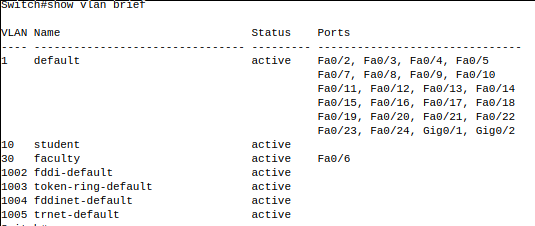
\includegraphics[width=.45\linewidth]{Figures/2020-03-19-180342_535x226_scrot.png}}\par
\subfloat[show ip int brief on Switch 3]{\label{Show13Ip3}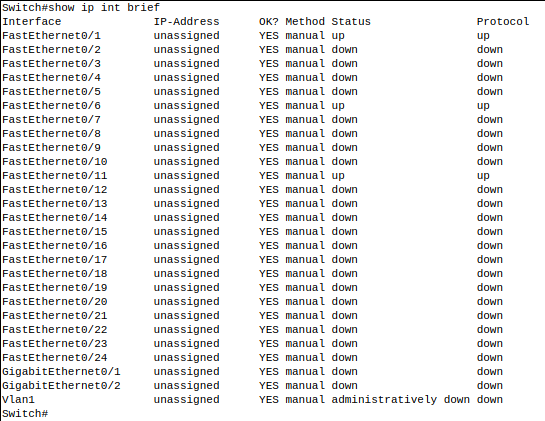
\includegraphics[width=.45\linewidth]{Figures/2020-03-19-180447_545x421_scrot.png}}\hfill
\subfloat[show vlan brief on Switch 3]{\label{Show13Vlan3}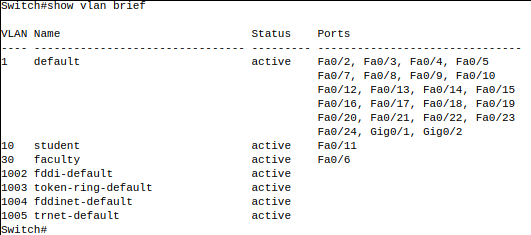
\includegraphics[width=.45\linewidth]{Figures/2020-03-19-180514_531x235_scrot.png}}\par
\caption{Switch Configurations}\label{Show13}
\end{figure}

The network is all up and running, We can now ping from PC3 to PC6 across the
same network.

\begin{figure}[!hbt]\centering
\subfloat[PC3 pinging PC6]{\label{Net13PC3}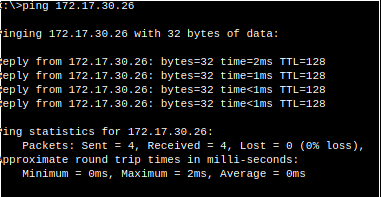
\includegraphics[width=.45\linewidth]{Figures/2020-03-19-181331_381x197_scrot.png}}\hfill
\subfloat[Layout of the Network]{\label{Net13Lay}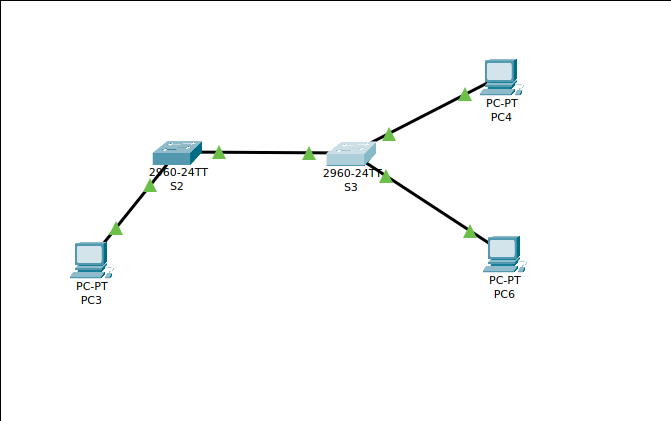
\includegraphics[width=.45\linewidth]{Figures/2020-03-08-183211_671x421_scrot.png}}\par 
\caption{The Network Connected}\label{Net13}
\end{figure}


%===================================

\end{document}
